\documentclass{beamer}
\usepackage{ctex}
\usepackage[utf8]{inputenc}
\usepackage{graphicx}
\usepackage{amsmath}
\usepackage{amssymb}
\usepackage{booktabs}
\usepackage{hyperref}
\usepackage{subcaption}
\usepackage{multicol}
\usepackage{listings}
\usepackage{multirow}
\usepackage{tabularx}

\bibliographystyle{alpha}


\usetheme{Madrid}
\usecolortheme{seahorse}

% 自定义块颜色
\setbeamercolor{block title}{bg=blue!30,fg=black}
\setbeamercolor{block body}{bg=blue!10,fg=black}
\setbeamercolor{alertblock title}{bg=red!50,fg=black}
\setbeamercolor{alertblock body}{bg=red!20,fg=black}

% 开启图表编号
\setbeamertemplate{caption}[numbered]

\title{\textbf{周报——向嘉豪(2024年12月17日)}}
\author{向嘉豪}
\institute{衡阳师范学院}
\date{2024年12月17日}

\begin{document}

\begin{frame}
    \titlepage
\end{frame}

\begin{frame}
    \frametitle{摘要}
    \begin{block}{本周主要工作}
        \begin{itemize}
            \item \textbf{摘要的修改与完善}
            \item \textbf{实验章节的改进}
        \end{itemize}
    \end{block}
 
\end{frame}

\section{摘要的修改与完善}

\begin{frame}
    \frametitle{摘要的修改与完善}
    在参考了\textit{IEEE Transactions on Computers}中相关文献\cite{Liu2020}后,我们对论文摘要进行了细致的调整:
    \begin{enumerate}
        \item 将摘要细分为多个小节,新增“动机”和“相关工作”两个部分。
        \item 在“动机”部分(见图\ref{fig:motivation}),详细阐述了研究问题的重要性和必要性。
        \item 在“相关工作”部分(见图\ref{fig:related_work}),对现有研究进行了系统综述,明确了本研究的创新点和贡献。
    \end{enumerate}
    \begin{figure}[h]
      \centering
      \begin{subfigure}[b]{0.3\textwidth}
        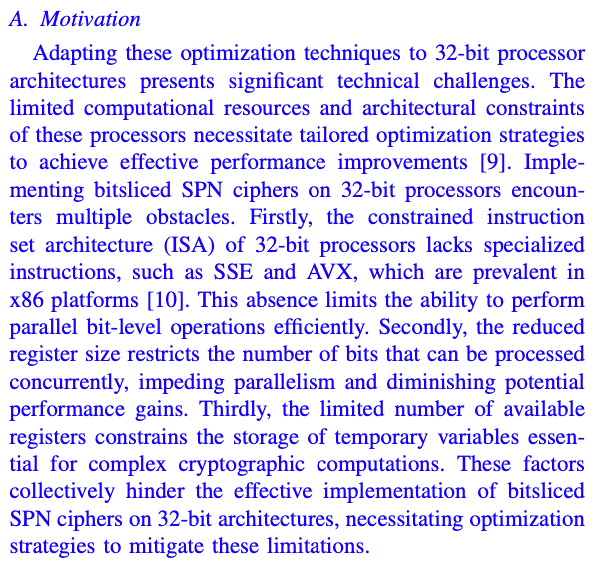
\includegraphics[width=\textwidth]{./fig/motivation.png}
        \caption{动机部分}
        \label{fig:motivation}
      \end{subfigure}
      \hfill
      \begin{subfigure}[b]{0.3\textwidth}
        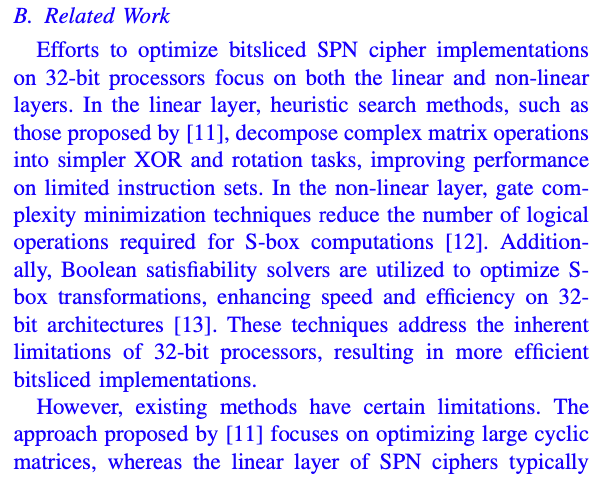
\includegraphics[width=\textwidth]{./fig/relatedWork.png}
        \caption{相关工作部分}
        \label{fig:related_work}
      \end{subfigure}
      \caption{摘要部分的修改}
      \label{fig:abstract_modifications}
    \end{figure}
\end{frame}

\section{实验章节的改进}

\begin{frame}
    \frametitle{实验章节的改进}
    为了提高实验部分的完整性和学术规范性,我们进行了以下改进:
    \begin{enumerate}
        \item 提供了实验测试的开源链接,方便他人重复实验并验证结果。
        \item 将表格格式由IEEE默认样式改为\cite{Liu2020}中使用的三线表,提升了表格的美观性和可读性。
        \item 增加了对实验结果的深入分析和解释(见图\ref{fig:experiment_analysis}),补充了非SPN结构的密码算法实现(见图\ref{fig:non_spn}),更充分地展示了研究成果。
    \end{enumerate}
    \begin{figure}[h]
      \centering
      \begin{subfigure}[b]{0.3\textwidth}
        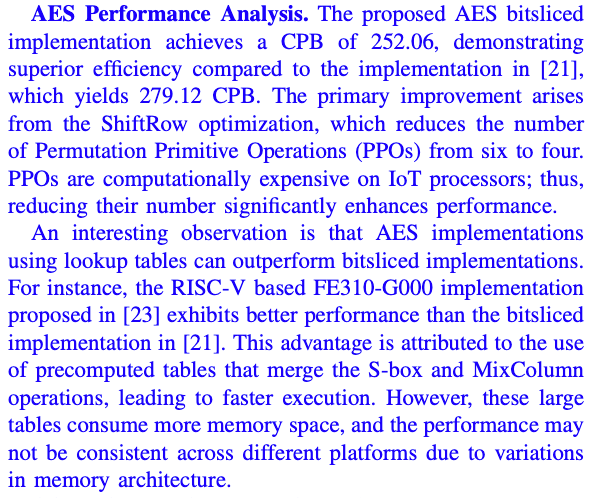
\includegraphics[width=\textwidth]{./fig/aseAnalysis.png}
        \caption{实验结果分析}
        \label{fig:experiment_analysis}
      \end{subfigure}
      \hfill
      \begin{subfigure}[b]{0.3\textwidth}
        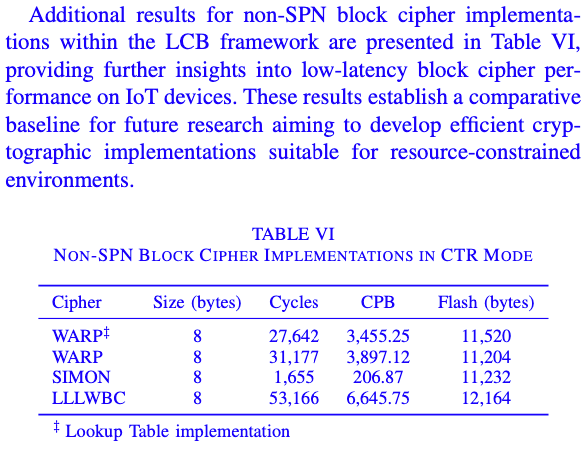
\includegraphics[width=\textwidth]{./fig/nonSPN.png}
        \caption{非SPN结构算法实现}
        \label{fig:non_spn}
      \end{subfigure}
      \caption{实验章节的改进}
    \end{figure}
\end{frame}

\begin{frame}[allowframebreaks]
    \frametitle{参考文献}
    \bibliography{../../paper}
\end{frame}

\begin{frame}
    \frametitle{老师评语}
    \begin{alertblock}{确定好可以投稿}
        好的
    \end{alertblock}

    \begin{block}{本周计划}
        \begin{itemize}
            \item 完成论文的最终校正和投稿。
            \item 开始筹备第三篇的工作。
        \end{itemize}
    \end{block}
\end{frame}

\end{document}